\section{Design Overview}\label{sec:design overview}

This section provides a high-level overview of our HOHS data-reduction framework. We present the overall framework in Figure~\ref{fig:overview}, followed by a summary of the SZ-based pipeline that serves as the foundation of SZ3-HOHS and MRCZ. We then introduce the preprocessing steps and design considerations for HOHS data that are applied across all compressors.

\begin{figure}[htb]
    \centering
    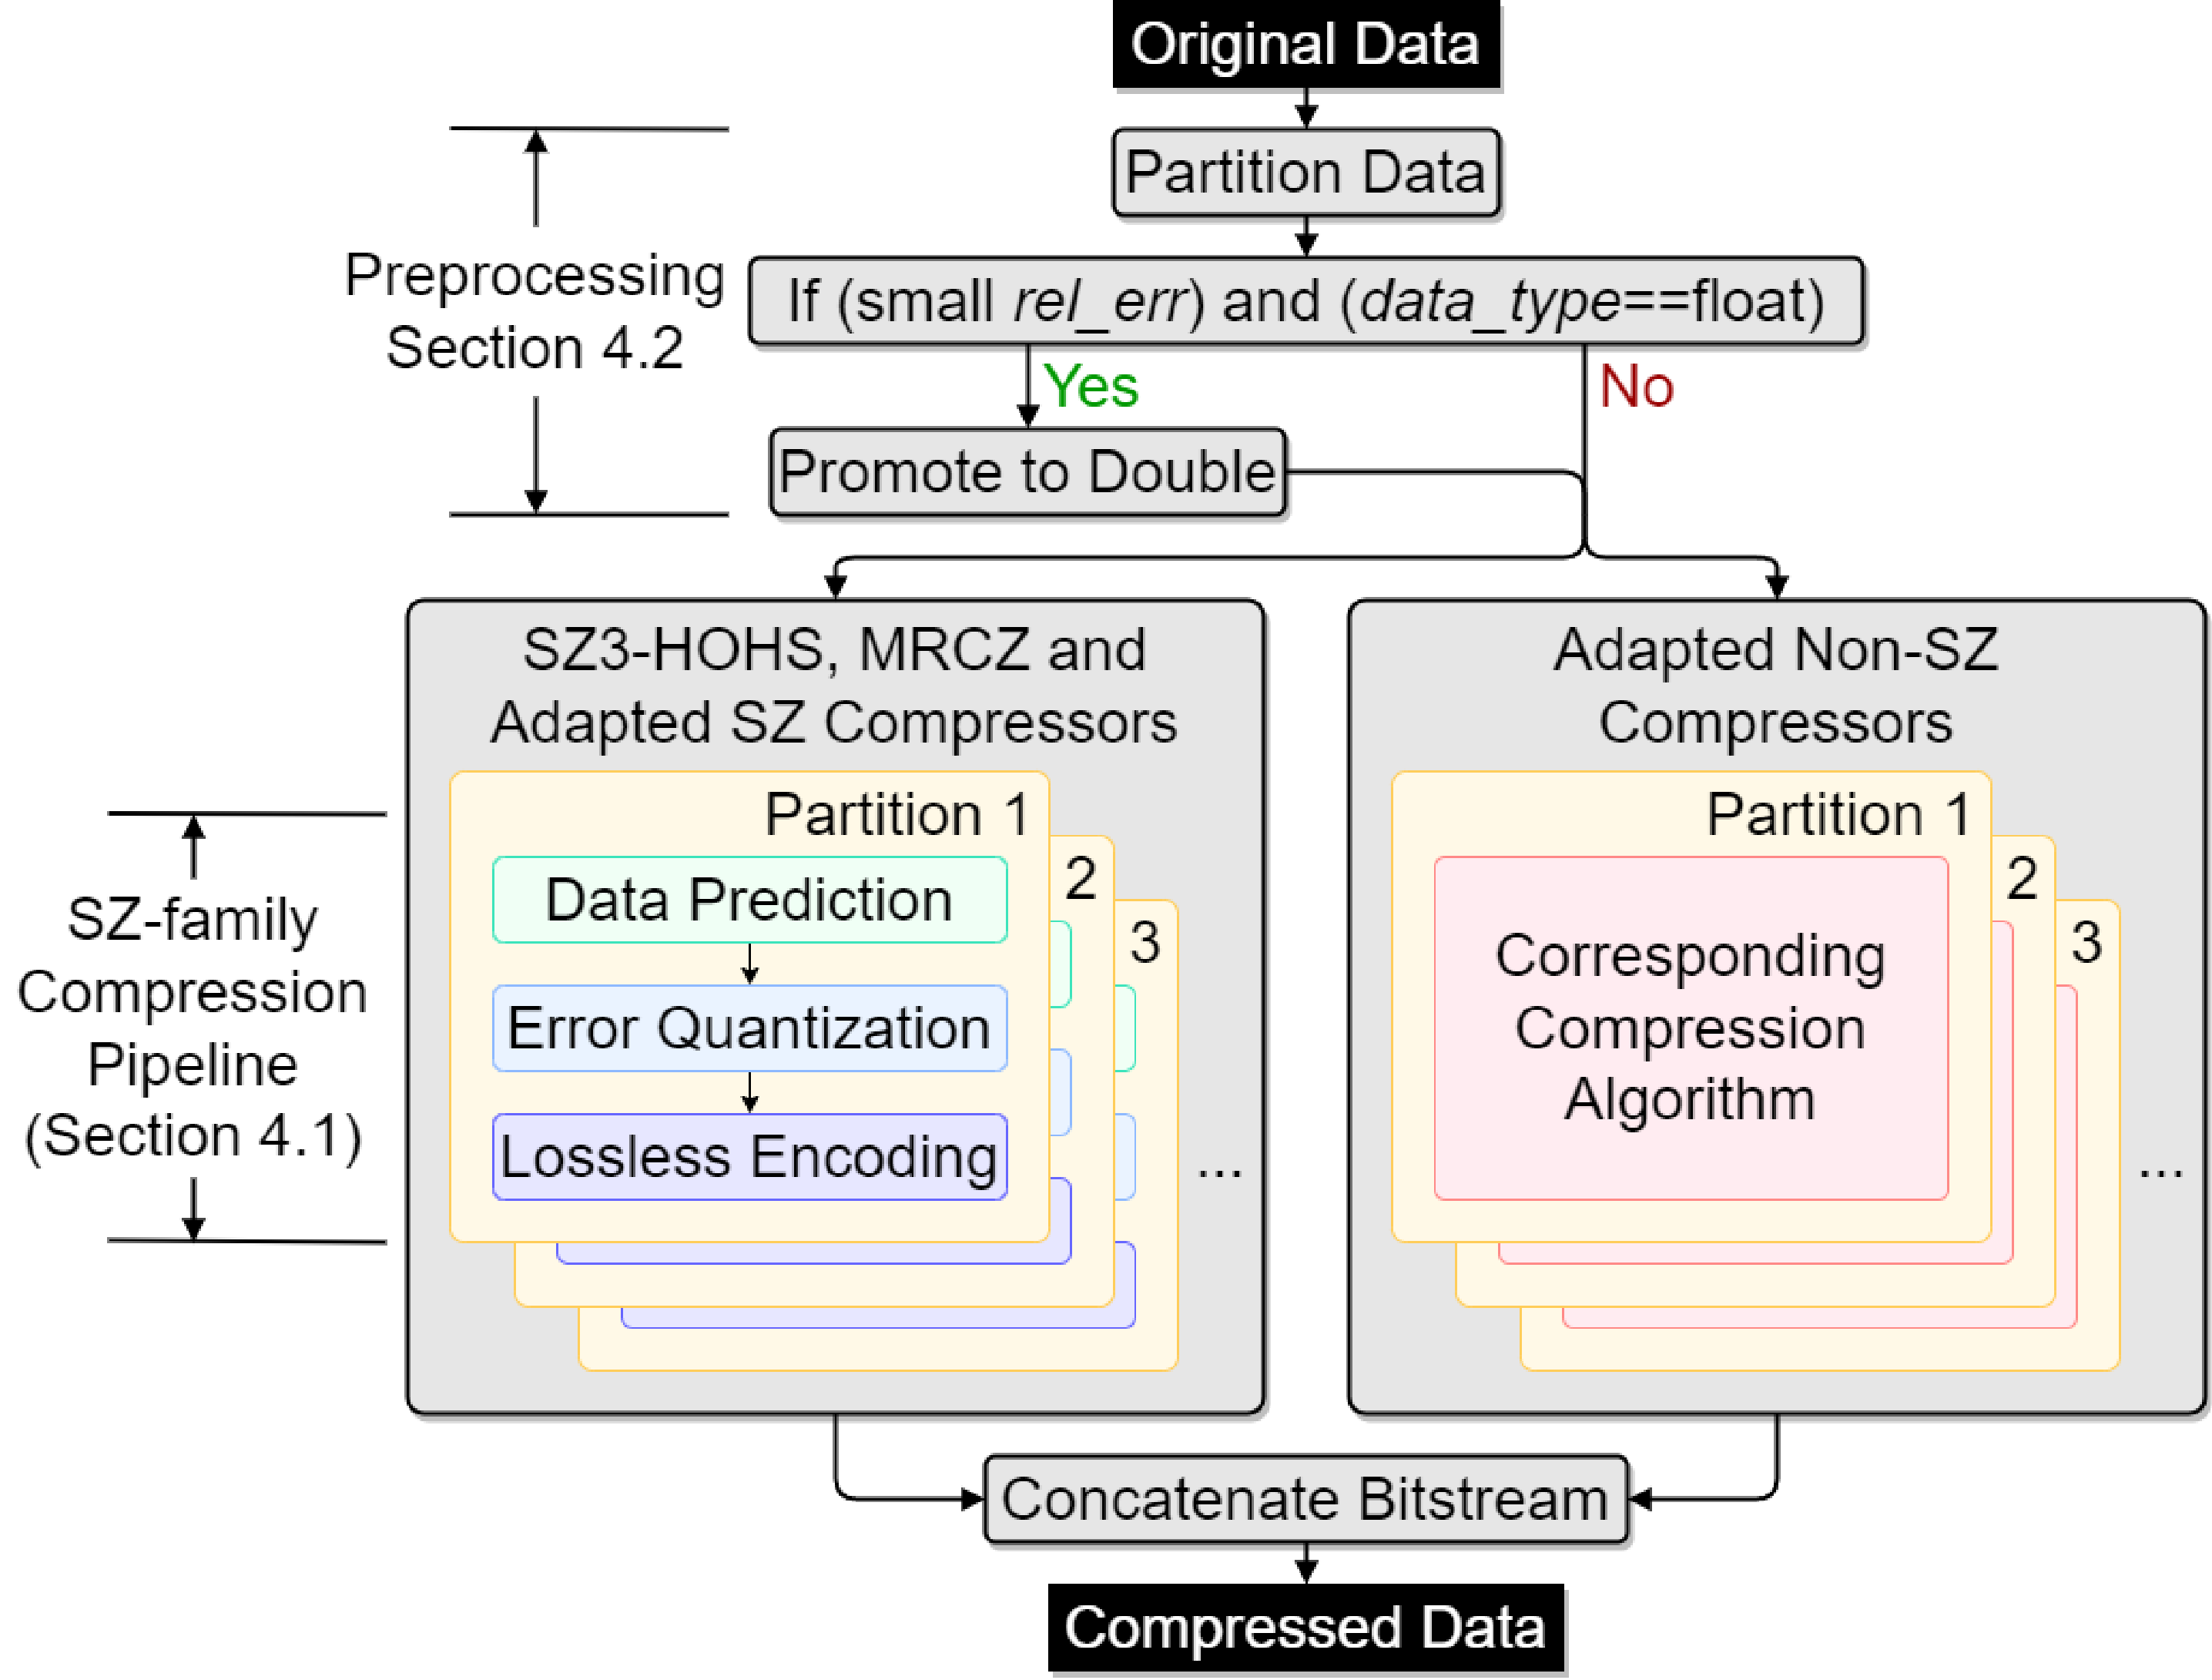
\includegraphics[width=\linewidth]{figs/4/Overall Framework.pdf}
    \caption{Overall Framework for HOHS Data Reduction}
    \label{fig:overview}
\end{figure}

\subsection{SZ-family Compression Pipeline}\label{sec:design overview:family}

Both SZ3-HOHS and MRCZ adopt the standard SZ-family compression pipeline~\cite{di2016fast,tao2017significantly,liang2018error,zhao2021optimizing,liang2022sz3}. As shown in Figure~\ref{fig:overview}, this pipeline follows a classic prediction-based model consisting of three main stages: \textit{data prediction}, \textit{error-bounded quantization} of prediction residuals, and \textit{lossless encoding} of the resulting quantization symbols. During prediction, each data value is estimated using a predictor constructed from available reference information. The difference between the original and predicted values is then quantized under a user-specified error bound, ensuring that the reconstructed data satisfy the prescribed pointwise error constraint. Finally, the resulting quantization symbols are encoded losslessly, typically using a combination of Huffman coding and Zstandard~\cite{zstd}.

Prediction accuracy is critical to the effectiveness of SZ-family compressors. More accurate prediction generally produces smaller residuals and causes the corresponding quantization symbols to concentrate around zero. The resulting lower-entropy distribution can be encoded more efficiently and therefore generally leads to a higher compression ratio. Existing SZ compressors employ different prediction strategies. SZ1~\cite{di2016fast}, SZ3~\cite{liang2022sz3,zhao2021optimizing}, and QoZ2.0~\cite{liu2024high} use iterative schemes, in which previously reconstructed values are used to predict subsequent data points. In contrast, SZ2~\cite{tao2017significantly} adopts a non-iterative, block-based regression approach that generates model coefficients, which are quantized and stored as auxiliary information for reconstruction.

In addition to their statistical distribution, local regularity and repeated patterns in the quantization-symbol sequence can further improve the effectiveness of subsequent lossless compression. Recent variants, including SZ3~\cite{liang2022sz3,zhao2021optimizing} and QoZ2.0~\cite{liu2024high}, incorporate optimizations that improve such regularity.

Within this common pipeline, SZ3-HOHS adopts an iterative prediction strategy consistent with SZ3-style designs~\cite{liang2022sz3,zhao2021optimizing}, whereas MRCZ employs a model-based prediction strategy that is conceptually closer to the non-iterative approach used in SZ2~\cite{tao2017significantly}. Our primary contribution is the development of prediction methods tailored to the structural characteristics of HOHS data.

\subsection{General Preprocessing for HOHS Data}

Two general preprocessing steps are applied to HOHS data for our developed methods and other methods to be evaluated in this paper. First, spectral elements in HOHS data are grouped into multiple partitions based on their ordering within each field, and each partition is processed independently by a separate OpenMP thread. This element-centric organization enables straightforward parallelization without introducing inter-thread dependencies, while also preserving contiguous memory access within each thread. Second, when the input data are stored in single-precision floating-point format, and very small relative error bounds are specified, numerical precision may become insufficient due to amplified round-off errors. In such cases, the input data are conditionally promoted to double precision.

\subsection{Element-local Design Considerations}

In our design, we restrict prediction to be element-local and do not explicitly exploit correlations across neighboring elements. This choice is motivated by three considerations.

\begin{enumerate}
\item \textit{Irregular Connectivity}: Elements in HOHS data are connected in an unstructured manner, and each element is associated with its own local coordinate system. Exploiting cross-element correlations would require identifying adjacent elements sharing a common face and aligning their orientations, which introduces computational complexity and non-trivial overhead.
\item \textit{Prediction Accuracy}: Although neighboring elements may exhibit physical correlations, exploiting them does not necessarily improve prediction accuracy. In our experiments, extending prediction across element boundaries often reduces prediction accuracy compared with element-local prediction. A detailed evaluation is provided in Section~\ref{sec:SZ3-HOHS:cross_element}.
\item \textit{Transform Locality}: The model-based transform used in MRCZ operates on data within individual elements, where the data naturally form tensor-product structures, which are not preserved across element boundaries, making it difficult to extend the transform consistently.
\end{enumerate}

